\documentclass{standalone}
\usepackage{amsmath}
\usepackage{amssymb}
\usepackage{tikz}
\usepackage{mathrsfs}
\usepackage{ifthen}

\newcommand{\perpp}{\perp\!\!\!\perp}
\DeclareMathOperator{\so}{\mathfrak{s}}
\DeclareMathOperator{\ra}{\mathfrak{r}}
\DeclareMathOperator{\supp}{supp}
\DeclareMathOperator{\id}{id}
\DeclareMathOperator{\dom}{dom}
\DeclareMathOperator{\ran}{ran}
\DeclareMathOperator{\Min}{Min}
\DeclareMathOperator{\cod}{cod}
\newcommand{\smallerthan}{<}
\newcommand{\greaterthan}{>}
\newcommand{\defeq}{:=}
\newcommand{\eqdef}{=:}

\newcommand{\cat}[1]{\textbf{#1}}
\DeclareMathOperator{\IG}{\mathscr{IG}}


\begin{document}
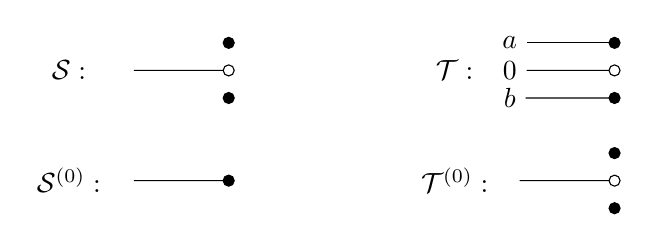
\begin{tikzpicture}[scale=0.7]
\node (SS0) at (0,0) {};
\draw[fill=black] ([shift={+(-0.1,0)}]SS0) circle (0.1);
\node (start_X) at ([shift={+(-2,-0.5)}]SS0) {};
\node (end_X) at ([shift={+(2,0)}]start_X) {};
\draw[-] (start_X)--(end_X);
\draw[fill=white] ([shift={+(-0.1,0)}]end_X) circle (0.1);
\node (Y1) at ([shift={+(0,-0.5)}]end_X) {};
\draw[fill=black] ([shift={+(-0.1,0)}]Y1) circle (0.1);
\node (start_S0) at ([shift={+(0,-2)}]start_X) {};
\node (end_S0) at ([shift={+(2,0)}]start_S0) {};
\draw[-] (start_S0)--(end_S0);
\draw[fill=black] ([shift={+(-0.1,0)}]end_S0) circle (0.1);

\node (S) at ([shift={+(-1,0)}]start_X) {$\mathcal{S}:$} ;
\node (S0) at ([shift={+(-1,0)}]start_S0) {$\mathcal{S}^{(0)}:$} ;

\node (start_a) at ([shift={+(5,0)}]SS0) {$a$};
\node (end_a) at ([shift={+(2,0)}]start_a)  {};
\draw[-] (start_a)--(end_a);
\draw[fill=black] ([shift={+(-0.1,0)}]end_a) circle (0.1);
\node (start_0) at ([shift={+(0,-0.5)}]start_a) {$0$} ;
\node (end_0) at ([shift={+(2,0)}]start_0)  {};
\draw[-] (start_0)--(end_0) ;
\draw[fill=white] ([shift={+(-0.1,0)}]end_0) circle (0.1);
\node (start_b) at ([shift={+(0,-0.5)}]start_0) {$b$} ;
\node (end_b) at ([shift={+(2,0)}]start_b)  {};
\draw[-] (start_b)--(end_b) ;
\draw[fill=black] ([shift={+(-0.1,0)}]end_b) circle (0.1);
\node (Y0) at ([shift={+(0,-1)}]end_b) {};
\draw[fill=black] ([shift={+(-0.1,0)}]Y0) circle (0.1);
\node (start_X) at ([shift={+(-2,-0.5)}]Y0) {};
\node (end_X) at ([shift={+(2,0)}]start_X) {};
\draw[-] (start_X)--(end_X);
\draw[fill=white] ([shift={+(-0.1,0)}]end_X) circle (0.1);
\node (Y1) at ([shift={+(0,-0.5)}]end_X) {};
\draw[fill=black] ([shift={+(-0.1,0)}]Y1) circle (0.1);

\node (T) at ([shift={+(-1,0)}]start_0) {$\mathcal{T}:$} ;
\node (T0) at ([shift={+(-1,0)}]start_X) {$\mathcal{T}^{(0)}:$} ;
\end{tikzpicture}\end{document}